\documentclass[parskip=full,11pt]{scrartcl}
\usepackage[utf8]{inputenc}

\title{\Huge Parkview\\
    \LARGE \normalfont Performance Dashboard for Continuous Benchmarking of HPC Libraries}
\author{Chingun Ariunbat, Jamil Bagga, Walter Alexander B\"ottcher,\\Darius Schefer, Maximilian Schik}

% section numbers in margins:
\renewcommand\sectionlinesformat[4]{\makebox[0pt][r]{#3}#4}

% header & footer
\usepackage{scrlayer-scrpage}
%\lofoot{\today} % Date in footer
\refoot{\today}  % no idea what this does
\pagestyle{scrheadings}

\usepackage[sfdefault,light]{roboto}
\usepackage[T1]{fontenc}
\usepackage[english]{babel}
\usepackage[yyyymmdd]{datetime} % must be after babel
\usepackage{float}
\renewcommand{\dateseparator}{-}
\usepackage[colorlinks=true, linkcolor=blue]{hyperref}
\usepackage{amsmath} % for $\text{}$
\usepackage[nameinlink]{cleveref}
\crefname{figure}{Abb}{Abb}
\usepackage[section]{placeins}
\usepackage{xcolor}
\usepackage[nonumberlist, toc]{glossaries}     % provides glossary commands, [toc] to appear in table of contents
\usepackage{graphicx}
\usepackage{dirtree}
\usepackage[width=2cm, filledcolor=green]{progressbar}
\graphicspath{ {./images/} }
\hypersetup{
	pdftitle={Design},
	bookmarks=true
}
\usepackage{QA}
\usepackage{csquotes} % provides \enquote{} command

\usepackage{booktabs}% http://ctan.org/pkg/booktabs
\newcommand{\tabitem}{~~\llap{\textbullet}~~}


\begin{document}

\maketitle
\begin{figure}[h]
	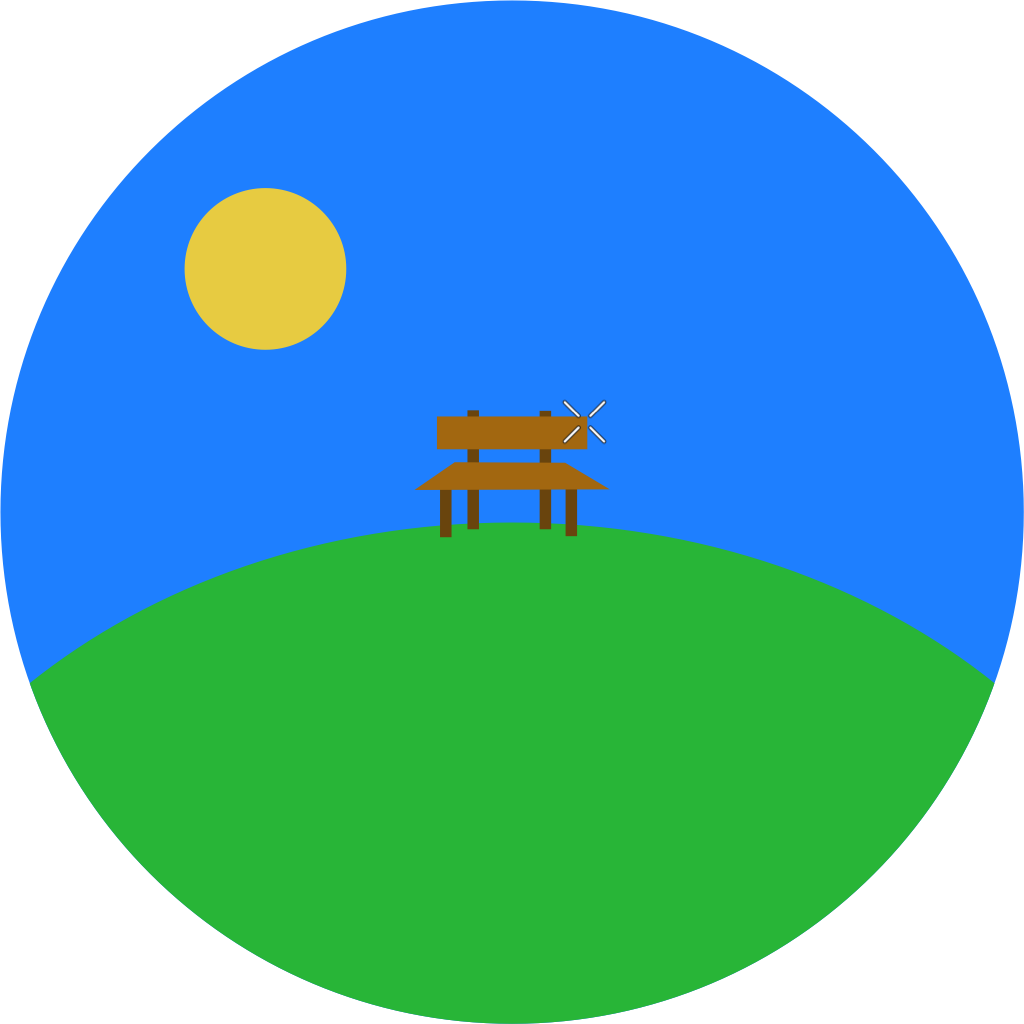
\includegraphics[width=11cm]{parkview.png}
	\centering
\end{figure}

\thispagestyle{empty}

\clearpage
\pagenumbering{arabic}

\tableofcontents
\clearpage

\section{Introduction}
This document describes in detail the quality assurance phase of \parkview{}, using automated unit tests for both the frontend and backend. This ensures that the implementation behaves according to the specification document.
\begin{itemize}
  \item The tests from the specification document are ran to check the functionality of the implementation
  \item Line and Branch coverage are given for relevant parts of the implementation
  \item A continuous integration pipeline is set up to check the functionality after changes are made.
\end{itemize}
\clearpage

\section{Scenarios}

\scenario{Inspecting Last Change}{scn:inspect_last_change}
{Ted: \Gls{user}, CI: \Gls{benchmarking system}}
{Ted works on a project that has \emph{PROJECT NAME} set up. He makes changes on a performance critical component. After that he pushes his changes to the repository. The CI sends its benchmark results to the system, which stores it in a persistent way. Ted opens the webapp and selects a benchmark. He sees a list of all recent changes. The changes without benchmark data are greyed out. Ted selects his newest change. He selects a device to take the benchmark data from. The change appears in a list of selected changes. Ted selects the \enquote{Create New Plot} option. A popup appears. Ted chooses the dimension he wants to inspect. After he configured his plot he decides to save the \gls{template} for later use. He selects the \enquote{Save Template} option. He enters a name for the \gls{template} and selects the \enquote{Save} option. After that he selects the \enquote{Generate Plot} option. Ted gets redirected to a new site where he can inspect his plot. He decides to send this plot to a coworker. He selects the \enquote{Share} option and a link gets displayed. He copies the link and sends it to his coworker.}

\scenario{Comparing Benchmarks}{scn:comp_benchmarks}
{Greta: \Gls{user}}
{Greta opens the webapp. She selects a benchmark. She selects two benchmarks by first picking a specific change and then a specific device. She opens the configuration popup by selecting the \enquote{Create New Plot} option. She wants to use a previously created \gls{template}. She selects the \enquote{Use Template} option and chooses her \gls{template} from a list of available ones. The settings specified in the \gls{template} get applied to the current \gls{configuration}. Greta makes final adjustments and then selects the \enquote{Generate Plot} option. After that she gets redirected to a new site where she can inspect her plot. Ted also wants to download the plot for use in his publication. He selects the \enquote{Export} option. He gets to choose between a seleciton of filetypes. He picks his preferred one. A link gets displayed leading to a download with the selected filetype.}

\scenario{Performance Tracking}{scn:perf_tracking}
{CI: \Gls{benchmarking system}}
{The CI runs a specific benchmark for a specific change on a specific device. It sends a POST request to the system containing the results and the benchmark type, change identification and device name. The system receives the results and stores them in a persistent database. It recognizes that the benchmark performance has dropped by a significant factor. The system triggers a hook that sends a message to the developer slack channel informing about the performance drop. It also publishes a comment under the change on GitHub.}


\clearpage

\section{Code Coverage Statistics}

\subsection{Frontend}


\begin{center}
  \begin{tabular}{llllllll}
    Package & LOC &  Line & &  Branch & & Method &  \\
    \midrule
    \covRow{app}{0}{0}{0}{0} \\
    \covRow{lib}{0}{0}{0}{0} \\
    \covRow{logic}{0}{0}{0}{0} \\
  \end{tabular}
\end{center}

\subsection{Backend}

\begin{center}
  \begin{tabular}{llllllll}
    Package & LOC & Line & &  Branch & & Method &  \\
    \midrule
    \covRow{processing}{123.345}{36}{17}{12} \\
    \covRow{> transforms}{0}{10}{10}{10} \\
    \covRow{benchmark}{0}{71}{61}{31} \\
    \covRow{rest}{0}{0}{0}{0} \\
    \covRow{git}{0}{0}{0}{0} \\
    \covRow{database}{0}{0}{0}{0} \\
    \covRow{> exposed}{0}{0}{0}{0} \\
  \end{tabular}
\end{center}

\clearpage

\section{Continuous Integration}

\subsection{Setup}
Github offers with Github Actions a service for the easy setup of continuous integration pipelines. It makes heavy use of modern technologies like virtualization and containerization. Since the repoistory for \parkview{} is hosted on Github, Github Actions is used for continuos integration. While the running of basic build and unit tests and the generation of test reports is quite trivial, the integration tests are more complex in their setup and functionality.

All integration tests are written in Python 3 and use Selenium as a web testing framework. Selenium allows us to interact with any webpage and can be used to automate a list of steps to fully test the functionality of the system. Any test cases that have to use the API offered by the backend alone make use of the requests\footnote{https://github.com/psf/requests} library for Python. It also uses the docker bindings\footnote{https://github.com/docker/docker-py} for Python for building, starting and stopping containers for the frontend and backend, since every test scenario should be run from the same starting point. Therefore every test consists of a setup and a run phase. In the setup phase any necessary actions before the actual test run take place, such as loading data into the database. The actual test run throws an exception if it fails.

\subsection{Test Run}
On startup the integration test suite builds container images for both the frontend and the backend. The backend is ran with an embedded PostgreSQL database, since it should be cleared with each restart anyway. Before each specific test run it restarts both containers to get the same conditions for every run. It then waits a configured amount of time to give the containers enough time to properly start up. Then it proceeds with the setup phase for each test, following with the run phase. It then proceeds to the next test scenario.

\subsection{Continuous Deployment}
To offer users a way to test new features and collect feedback from them we set up a small webserver. We use continuous deployment to keep that instance constantly up to date and catch bugs and possible enhancements early. The keys to that are the container images that get build by the continuous integration pipeline. After the container images are built the webserver gets notified. It then pulls the new images and and restarts the services.

\clearpage

\section{Issues}

\subsection{Fixed Issues}
\fixed{Github Api for branches is paginated}
{Github returns the branches paged when using the Branches Api. Therefore the branch list on the frontend is incomplete.}
{When using the Github Api for retrieving branches, keep increasing the page number until no more branches are returned.}

\fixed{ConcurrentModificationException}
{Sometimes the backend throws a \texttt{ConcurrentModificationException}, while there isn't any way to reproduce this reliably, it might be an issue with an access from one thread that changes the linked lists used for caching the benchmark results while another thread is iterating over it.}
{Adding the \texttt{@Synchronized} annotation the functions handling the caching.}

\fixed{Invalid values for Performance Profile}
{The Performance Profile for Spmv benchmarks has invalid values for $x \leq 1$.}
{Filtering formats that haven't completed and filtering any values that are smaller than 1.}

\subsection{Open Issues}

\subsubsection{Frontend}

\issue{Template Management Page}
{Templates may introduce a necessity for a more powerful manipulation tool than the sidebar - like deleting, selecting a template first, and only selecting data points after that, manipulating them and other configuration. \\
Ideally this would be done on a separate page implemented specifically for template management.}

\issue{More Information on Plot Pages}
{Currently there is no information about which commits and devices are displayed in the plot on the plot page.}

\issue{Axis Scaling in Cookies}
{A minor quality of life improvement would be to store the currently selected axis scaling (linear / logarithmic) in the browser's cookies, as to make switching between multiple plots of the same type more seamless.}

\issue{Sensible Defaults for Axis Scaling}
{Axes should default to linear scaling instead of logarithmic for Performance Profiles.}

\issue{Reuse Current Plot Settings when opening another Plot}
{When on a plot page, selecting \enquote{Configure Plot} should open the configuration pop-up with the current plot settings instead of the defaults to make subsequent changes to the plot configuration simpler.}

\issue{Disable Plot Button when no Plots are available}
{Currently the plot button is enabled even if there are no available plots conforming to the user selection. Pressing it leads to an empty plot page.}

\subsubsection{Backend}

\issue{Preconditioner Plots}
{Plots for Preconditioner Benchmarks are still missing but shouldn't be a lot of effort to implement later on due to the modular nature of the backend.}

\issue{HikariCP}
{Every time the backend is started, HikariCP logs a warning message, however, it doesn't seem to affect any functionality. This might just be a minor oversight in a configuration file somewhere.}

\issue{POST Authentication}
{Currently there is no form of authentication required to POST data to the backend. This might be desirable once \parkview{} is hosted in a public network to prevent malicious requests.}

\subsubsection{Miscellaneous}

\issue{NGINX}
{The container for the frontend currently uses \texttt{ng serve} which is less than desirable for production use. Ideally the frontend container should use NGINX as an actual webserver.}

\clearpage


\appendix

%TBA

\end{document}
